\documentclass[12pt, a4paper]{article}

\usepackage{tikz}
\usetikzlibrary{shapes.geometric}    % trapezium
\usetikzlibrary{arrows}              % arrow tips
\usepackage{amsmath, amsfonts}
\usepackage{bm}                      % boldsymbol
\usepackage{makecell}                % makecell
\usetikzlibrary{matrix,calc}
\usepackage{color}
\usepackage{xcolor}
\usepackage{multicol}
\definecolor{mygray}{HTML}{F0F0F0}
\definecolor{myred}{HTML}{CD594A} 
\definecolor{mygreen}{HTML}{829356} 
\definecolor{myblue}{HTML}{3C6478} 
\usepackage{mathtools}
\usetikzlibrary{decorations.pathreplacing}

\newcommand{\trans}{\text{T}}
\newcommand{\inv}{{-1}}
\newcommand{\eins}{\mathds{1}}
\DeclareMathOperator{\E}{\mathbb{E}}
\DeclareMathOperator{\I}{\mathbb{I}}
\newcommand{\tbf}[1]{\textbf{#1}}
\DeclareMathOperator{\tr}{tr}
\newcommand{\D}{\mathbf{D}}
\newcommand{\K}{\mathbf{K}}

\definecolor{mygray}{HTML}{F0F0F0}

\begin{document}




\begin{figure}[h!]
  \begin{minipage}{0.5\linewidth}
    \centering
    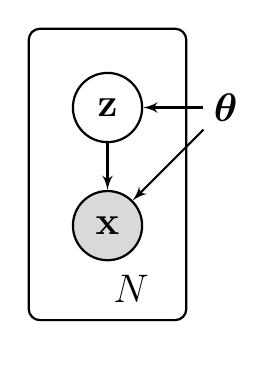
\begin{tikzpicture}[baseline=2, >=latex',thick] 
      \node [draw=black, circle, minimum size=25pt, name=z] at (0,0) {\Large{$\tbf{z}$}}; 
      \node [draw=black, fill=gray!30, circle, minimum size=25pt, name=x] at (0,-1.5)
      {\Large{$\tbf{x}$}}; 
      \draw [rounded corners] (-1, 1) rectangle (1, -2.7) {};
      \node at (0.3, -2.3) {\Large{$N$}};
      \node at (0,-3) {};
      
      \node [name=theta] at (1.5,0) {\Large{$\bm{\theta}$}};
      
      
      \draw [->] (z) -- (x);
      \draw [->] (theta) -- (z);
      \draw [->] (theta) -- (x);
      
    \end{tikzpicture}~\\
    \textbf{a) Generative Process} $p_{\bm{\theta}} (\tbf{z}) p_{\bm{\theta}} (\tbf{x}|\tbf{z})$
  \end{minipage}
  \begin{minipage}{0.5\linewidth}
    \centering
    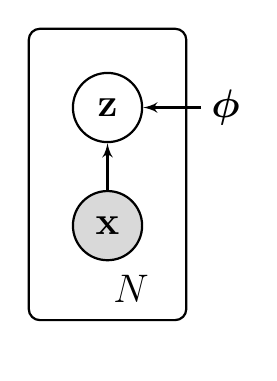
\begin{tikzpicture}[baseline=0, >=latex',thick] 
      \node [draw=black, circle, minimum size=25pt, name=z] at (0,0) {\Large{$\tbf{z}$}}; 
      \node [draw=black, fill=gray!30, circle, minimum size=25pt, name=x] at (0,-1.5)
      {\Large{$\tbf{x}$}}; 
      \draw [rounded corners] (-1, 1) rectangle (1, -2.7) {};
      \node at (0.3, -2.3) {\Large{$N$}};
      \node at (0,-3) {};

      \node [name=phi] at (1.5,0) {\Large{$\bm{\phi}$}};

      \draw [->] (phi) -- (z);
      \draw [->] (x) -- (z);
    \end{tikzpicture}~\\
    \textbf{b) Variational Approximation} $q_{\bm{\phi}} (\tbf{z}|\tbf{x})$
  \end{minipage}
\end{figure}
\end{document}
